\documentclass[tikz,border=12pt]{standalone}
\usepackage{fontspec}
\newfontfamily\hebrewfont[Script=Hebrew]{Noto Serif Hebrew}
\newcommand{\heb}[1]{{\hebrewfont #1}}
\newfontfamily\igfont[Ligatures=TeX]{Noto Serif}
\newcommand{\igtext}[1]{{\igfont #1}}
\usepackage{amsmath,amssymb}
\usetikzlibrary{positioning,arrows,shapes,fit,calc,backgrounds,decorations.pathreplacing}
\begin{document}
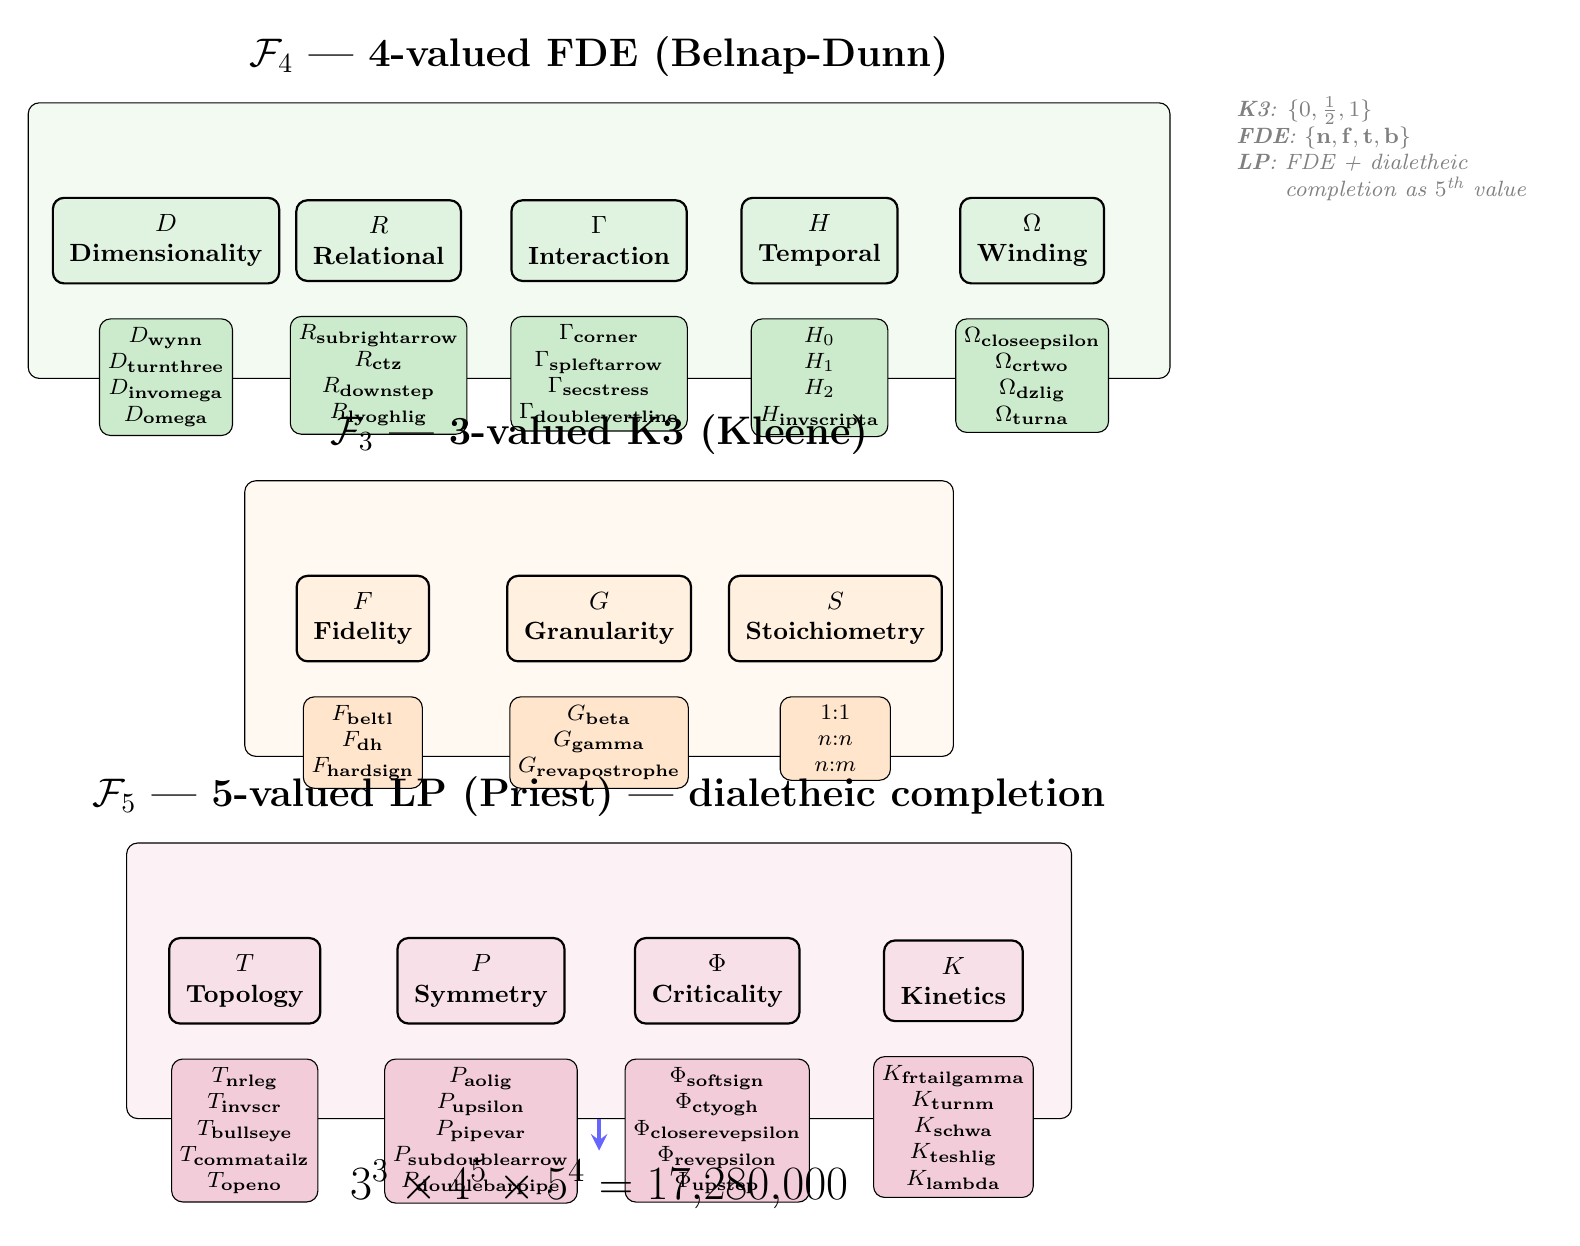
\begin{tikzpicture}[
  primnode/.style={rectangle,draw,thick,rounded corners,fill=#1!12,inner sep=6pt,align=center,minimum width=1.6cm,font=\small\bfseries},
  valnode/.style={rectangle,draw,rounded corners,fill=white,inner sep=3pt,font=\footnotesize,align=center,minimum width=1.4cm},
  valsel/.style={rectangle,draw,rounded corners,fill=#1!20,inner sep=3pt,font=\footnotesize\bfseries,align=center,minimum width=1.4cm},
  arr/.style={->,>=stealth,thick},
  tierbg/.style={rectangle,draw,rounded corners,fill=#1!5,inner sep=6pt},
]

% === 4-family primitives (FDE) ===
\node[tierbg=green!60!black,minimum width=14.5cm,minimum height=3.5cm] (f4) at (0,0) {};
\node[font=\Large\bfseries,above=0.2cm of f4] {$\mathcal{F}_4$ — 4-valued FDE (Belnap-Dunn)};

\node[primnode=green!60!black] (D) at (-5.5,0)  {$D$\\Dimensionality};
\node[primnode=green!60!black] (R) at (-2.8,0)  {$R$\\Relational};
\node[primnode=green!60!black] (Gam) at (0,0)  {$\Gamma$\\Interaction};
\node[primnode=green!60!black] (H) at (2.8,0)   {$H$\\Temporal};
\node[primnode=green!60!black] (Om) at (5.5,0)  {$\Omega$\\Winding};

% Values for each FDE primitive
\node[valsel=green!60!black,below=0.43cm of D] (Dvals)  {$D_{\text{wynn}}$\\$D_{\text{turnthree}}$\\$D_{\text{invomega}}$\\$D_{\text{omega}}$};
\node[valsel=green!60!black,below=0.43cm of R] (Rvals)  {$R_{\text{subrightarrow}}$\\$R_{\text{ctz}}$\\$R_{\text{downstep}}$\\$R_{\text{lyoghlig}}$};
\node[valsel=green!60!black,below=0.43cm of Gam] (Gamvals) {$\Gamma_{\text{corner}}$\\$\Gamma_{\text{spleftarrow}}$\\$\Gamma_{\text{secstress}}$\\$\Gamma_{\text{doublevertline}}$};
\node[valsel=green!60!black,below=0.43cm of H] (Hvals)  {$H_0$\\$H_1$\\$H_2$\\$H_{\text{invscripta}}$};
\node[valsel=green!60!black,below=0.43cm of Om] (Omvals) {$\Omega_{\text{closeepsilon}}$\\$\Omega_{\text{crtwo}}$\\$\Omega_{\text{dzlig}}$\\$\Omega_{\text{turna}}$};

% === 3-family primitives (K3) ===
\node[tierbg=orange,minimum width=9cm,minimum height=3.5cm] (f3) at (0,-4.8) {};
\node[font=\Large\bfseries,above=0.2cm of f3] {$\mathcal{F}_3$ — 3-valued K3 (Kleene)};

\node[primnode=orange] (F) at (-3,-4.8)  {$F$\\Fidelity};
\node[primnode=orange] (G) at (0,-4.8)   {$G$\\Granularity};
\node[primnode=orange] (S) at (3,-4.8)   {$S$\\Stoichiometry};

\node[valsel=orange,below=0.43cm of F] (Fvals)  {$F_{\text{beltl}}$\\$F_{\text{dh}}$\\$F_{\text{hardsign}}$};
\node[valsel=orange,below=0.43cm of G] (Gvals)  {$G_{\text{beta}}$\\$G_{\text{gamma}}$\\$G_{\text{revapostrophe}}$};
\node[valsel=orange,below=0.43cm of S] (Svals)  {$1{:}1$\\$n{:}n$\\$n{:}m$};

% === 5-family primitives (LP) ===
\node[tierbg=purple,minimum width=12cm,minimum height=3.5cm] (f5) at (0,-9.4) {};
\node[font=\Large\bfseries,above=0.2cm of f5] {$\mathcal{F}_5$ — 5-valued LP (Priest) — dialetheic completion};

\node[primnode=purple] (T) at (-4.5,-9.4)  {$T$\\Topology};
\node[primnode=purple] (P) at (-1.5,-9.4)  {$P$\\Symmetry};
\node[primnode=purple] (Phi) at (1.5,-9.4) {$\Phi$\\Criticality};
\node[primnode=purple] (K) at (4.5,-9.4)   {$K$\\Kinetics};

\node[valsel=purple,below=0.43cm of T] (Tvals)  {$T_{\text{nrleg}}$\\$T_{\text{invscr}}$\\$T_{\text{bullseye}}$\\$T_{\text{commatailz}}$\\$T_{\text{openo}}$};
\node[valsel=purple,below=0.43cm of P] (Pvals)  {$P_{\text{aolig}}$\\$P_{\text{upsilon}}$\\$P_{\text{pipevar}}$\\$P_{\text{subdoublearrow}}$\\$P_{\text{doublebarpipe}}$};
\node[valsel=purple,below=0.43cm of Phi] (Phivals) {$\Phi_{\text{softsign}}$\\$\Phi_{\text{ctyogh}}$\\$\Phi_{\text{closerevepsilon}}$\\$\Phi_{\text{revepsilon}}$\\$\Phi_{\text{upstep}}$};
\node[valsel=purple,below=0.43cm of K] (Kvals)  {$K_{\text{frtailgamma}}$\\$K_{\text{turnm}}$\\$K_{\text{schwa}}$\\$K_{\text{teshlig}}$\\$K_{\text{lambda}}$};

% Computation arrow
\node[below=0.4cm of f5,font=\LARGE] (total) {$3^3 \times 4^5 \times 5^4 = 17{,}280{,}000$};
\draw[->,>=stealth,ultra thick,blue!60] (f5.south) -- (total);

% Right-side annotation
\node[font=\footnotesize\itshape,text=gray,anchor=north west] at ($(f4.north east)+(0.5,0.2)$) {
\begin{tabular}{l}
\textbf{K3}: $\{0,\tfrac12,1\}$\\
\textbf{FDE}: $\{\mathbf{n},\mathbf{f},\mathbf{t},\mathbf{b}\}$\\
\textbf{LP}: FDE + dialetheic\\
\qquad completion as $5^{\text{th}}$ value
\end{tabular}};

\end{tikzpicture}
\end{document}
